\documentclass{beamer}
\usepackage[spanish]{babel}
\usepackage[utf8]{inputenc}
\usepackage{lmodern} % para cualquier tamaño de letra
\usepackage{amsmath}
\usepackage{amsfonts}
\usetheme{Copenhagen}
\setbeamercovered{transparent=30}

\begin{document}

\title{Compresión JPEG}
\author{Balbi Pablo Luis, Pazos Méndez Nicolás Javier}
\date{\today}

\begin{frame}
    \titlepage
\end{frame}

\section{El método de compresión JPEG}
\begin{frame}
    \frametitle{El método de compresión JPEG}
        Cuatro pasos fundamentales:
        \begin{enumerate}
            \item Separar la imagen en cuadrados de $8 \times 8$
            \item Aplicar la DCT\footnote{transformada del coseno discreta} a cada cuadrado
            \item Cuantizar los coeficientes del paso anterior
            \item Comprimir el conjunto de coeficientes finales
        \end{enumerate}

\end{frame}

\subsection{Separar la imagen en cuadrados de 8 x 8}

\begin{frame}
    % la imagen se divide así...
    \frametitle{1. Separar la imagen en cuadrados de $8 \times 8$}
    \begin{minipage}[t]{0.48\linewidth}
        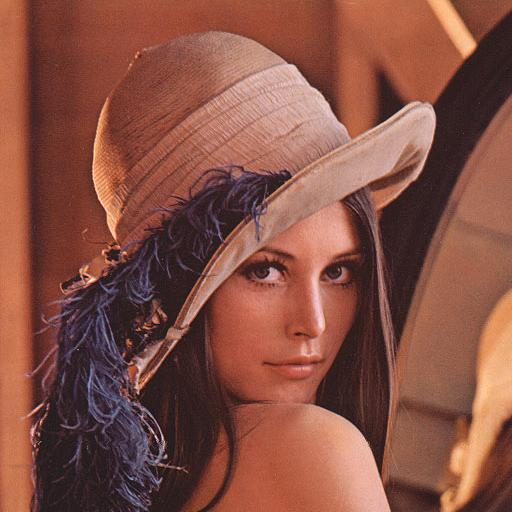
\includegraphics[width=5cm, height=5cm]{fig/lena.jpg}
    \end{minipage}
    \hfill
    \begin{minipage}[t]{0.48\linewidth}
        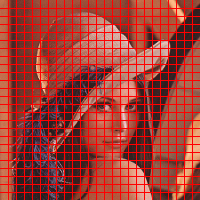
\includegraphics[width=5cm, height=5cm]{fig/lena_blocks.png}
    \end{minipage}
\end{frame}

\begin{frame}
    % explicar por qué partimos la imagen, y por qué no aplicamos la DCT a la imagen completa
    % \frametitle{Separar la imagen en cuadrados de $8 \times 8$}
    \textbf{¿Por qué partir la imagen en bloques?}
    \begin{itemize}
        \item Aplicar la DCT a la imagen completa requiere más memoria y es menos modular. % sirve que sea modular para cosas tipo GPU
        \item Las imágenes no suelen ser completamente homogéneas. Analizar las frecuencias de la imagen completa no es lo mejor para comprimir.
    \end{itemize}
\end{frame}

\begin{frame}
    % ya mencionamos (supuestamente...) que el método de JPEG se basa
    % en trabajar en el espacio de frecuencias, y 'descartar' frecuencias
    % que no sean muy relevantes.

    % qué pasa si usamos la DCT para comprimir sobre la imagen completa?
    % esta imagen no es homogénea, y las frecuencias de cada una de las 4 partes
    % es muy distinta a las demás. Para terminar de formar uno de los cuartos
    % de forma razonable se necesitan muchísimas frecuencias altas que vayan
    % anulando cosas donde corresponda.

    % si dividimos en partes (8x8 en este caso) podemos tratar diferente
    % a las frecuencias de cada bloque, y reconstruimos la imagen por partes
    % \frametitle{Separar la imagen en cuadrados de $8 \times 8$}
    \textbf{Usando la DCT sobre la imagen completa}

    Reconstrucción de una imagen utilizando la mitad de los coeficientes de su DCT (los de mayores frecuencias).

    \begin{minipage}[t]{0.4\linewidth}
        \begin{center}
            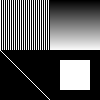
\includegraphics[scale=1.25]{fig/no_homogenea.png}\\         Original
        \end{center}
    \end{minipage}
    \hfill
    \begin{minipage}[t]{0.4\linewidth}
        \begin{center}
            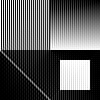
\includegraphics[scale=1.25]{fig/no_homogenea_comprimida.png}\\
            Reconstruida
        \end{center}
    \end{minipage}

\end{frame}

\begin{frame}
    \begin{center}
        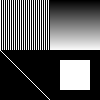
\includegraphics[scale=2]{fig/no_homogenea.png}
    \end{center}
\end{frame}
\begin{frame}
    \begin{center}
        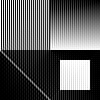
\includegraphics[scale=2]{fig/no_homogenea_comprimida.png}
    \end{center}
\end{frame}


\subsection{Aplicar la DCT a cada cuadrado}
\begin{frame}
    % ahora a cada bloque le hacemos...
    % abajo se ve un ejemplo de un bloque de 8x8 shifteado, y a la derecha
    % sus DCT. acá ya se ve algo que nos gusta. la DCT parecería ser reduntante
    \frametitle{2. Aplicar la DCT a cada cuadrado}
    \begin{itemize}
        \item \textit{Shiftear} los 64 valores de [0..255] a [$-$128..127].
        \item Aplicar la DCT al cuadrado.
    \end{itemize}

    % 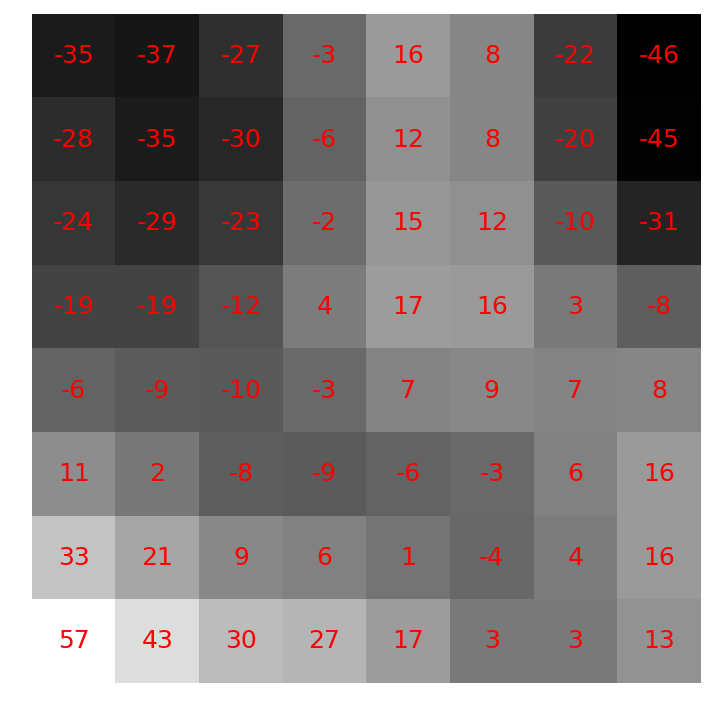
\includegraphics[scale=0.2]{fig/8x8random.png}
    % 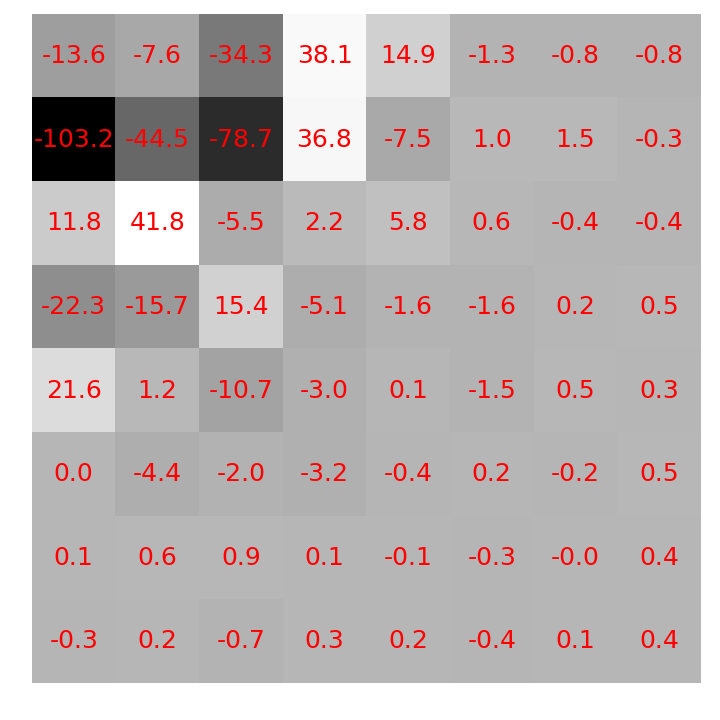
\includegraphics[scale=0.2]{fig/8x8random_dct.png}
\end{frame}

\begin{frame}
    \begin{center}
        \textbf{¿Cómo era la DCT?} Sea $I$ una imagen de $NM$ pixels
        \vspace{1cm}

        $F(u,v)=\frac{1}{NM}C(u)C(v)\,\sum_{x=0}^{7} \sum_{y=0}^{7}\,I(x,y)\,B(u,v,x,y)$

        \vspace{3mm}
        $f(x,y)=\frac{1}{NM}\,\sum_{x=0}^{7} \sum_{y=0}^{7}\,C(u)C(v)\,F(u,v)\,B(u,v,x,y)$

        \vspace{3mm}
        donde
        \vspace{3mm}

        $B(u,v,x,y) = cos\frac{(2x+1)u\pi}{2N}cos\frac{(2y+1)v\pi}{2M}$
        \[
        C(j) =
             \begin{cases}
                 \frac{1}{\sqrt{2}}\text{ si $j=0$}\\
                 1 \text{ sino}\\
             \end{cases}
        \]
        %NOTE: Quizas meter aca un "si la comparamos con la DFT no es tan diferente, escribiendo
        %ambas"
    \end{center}
\end{frame}


\begin{frame}
    % la DCT son los coeficientes de la combinación lineal de esta base (en 8x8)
    % que forma la imagen original. es la misma idea que en Fourier
    \begin{center}
        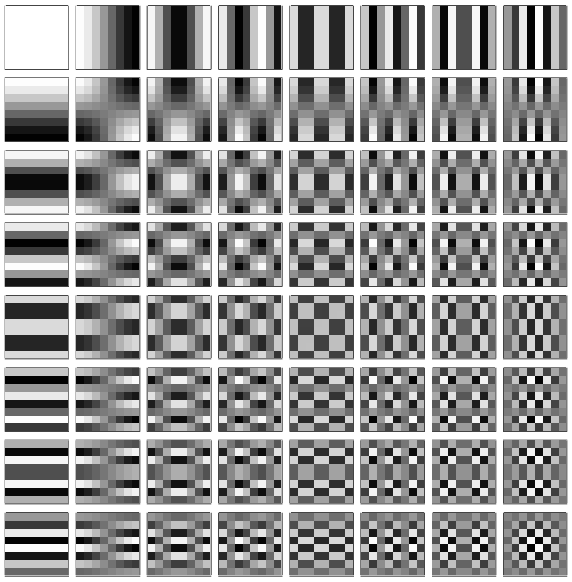
\includegraphics[scale=0.4]{fig/dctbase.png}
    \end{center}
\end{frame}

\begin{frame}
    % por qué nos sirve la DCT? ...
    % \frametitle{Aplicar la DCT a cada cuadrado}
    \textbf{¿Por qué nos sirve este espacio?}
    \begin{itemize}
        \item Para el ojo humano, las frecuencias bajas cargan más información que las altas $\rightarrow$ guardamos lo que más importa.
        \item Las imágenes con las que tratamos no suelen tener frecuencias altas: muchos coeficientes `nulos' $\rightarrow$ fácil codificación.
    \end{itemize}
\end{frame}

\begin{frame}
    % acá podemos ver ejemplos de distintos bloques de 8x8 y sus dct abajo.
    % puede verse cómo cuando la imagen es más 'suave' los coeficientes de
    % las frecuencias bajas son los de mayor magnitud.
    % en las imágenes con las que tratamos, los bloques suaves son mucho más
    % comunes, y los bloques no tan suaves no tiene mucha información de interés.
    % vamos a estar trabajando con muchas cosas de la pinta del último DCT que se
    % ve aquí

    % para que recordemos y nos refiramos más adelante, al primero coeficiente
    % se le llama DC, y a los demás AC

    % \frametitle{Aplicar la DCT a cada cuadrado}
    \textbf{Bloques de 8 x 8 y sus DCT}

    \begin{center}
        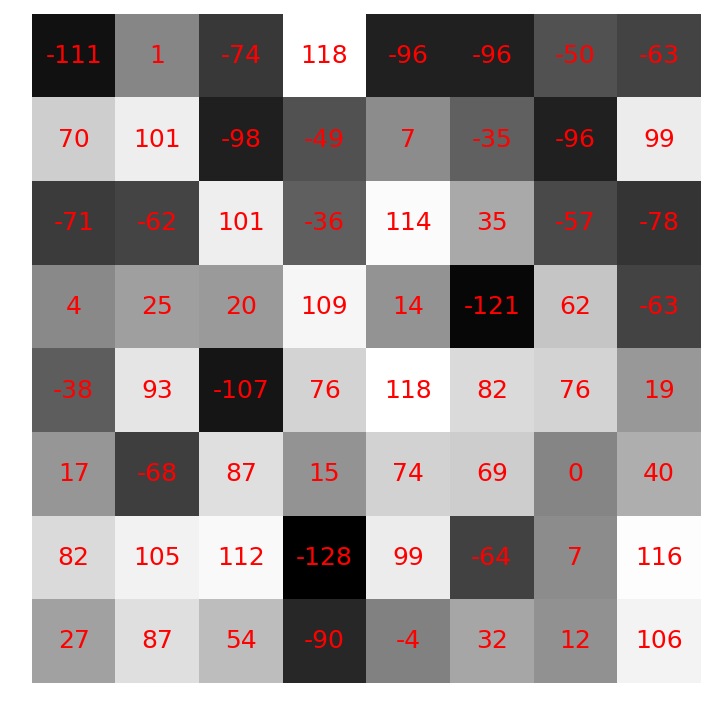
\includegraphics[scale=0.12]{fig/8x8random0.png}
        \hspace{0.5cm}
        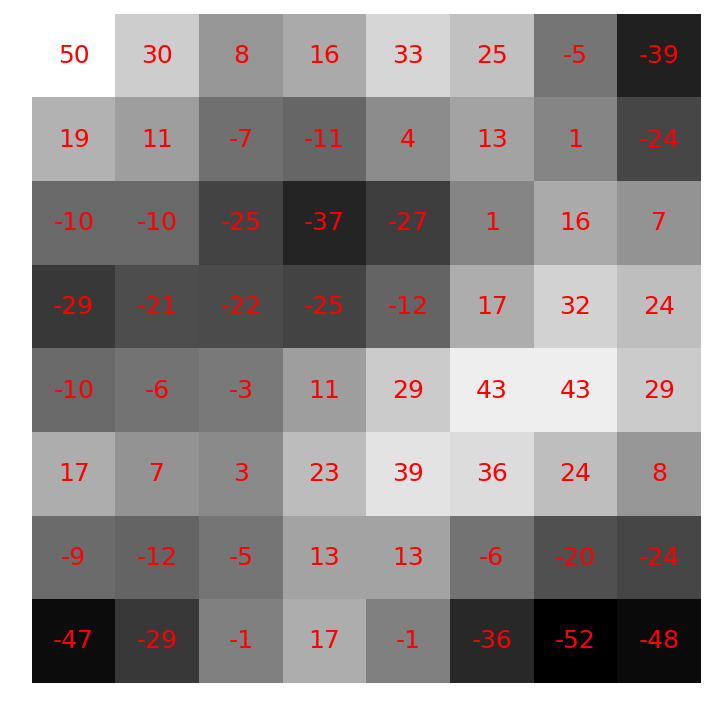
\includegraphics[scale=0.12]{fig/8x8random1.png}
        \hspace{0.5cm}
        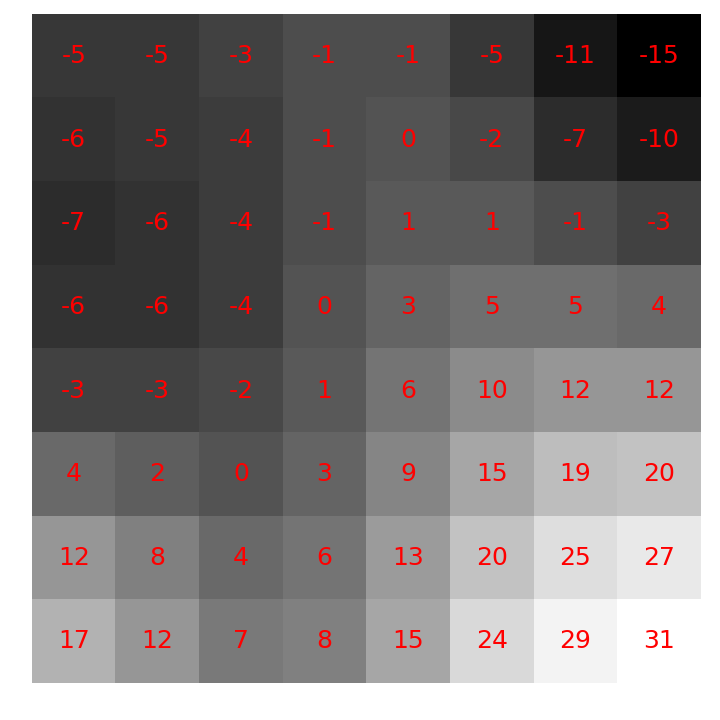
\includegraphics[scale=0.12]{fig/8x8random2.png}

        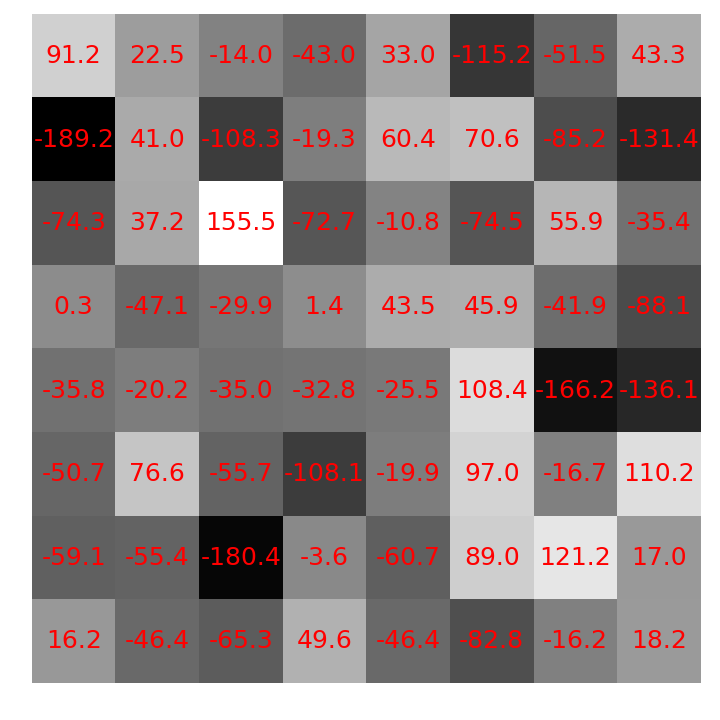
\includegraphics[scale=0.12]{fig/8x8random_dct0.png}
        \hspace{0.5cm}
        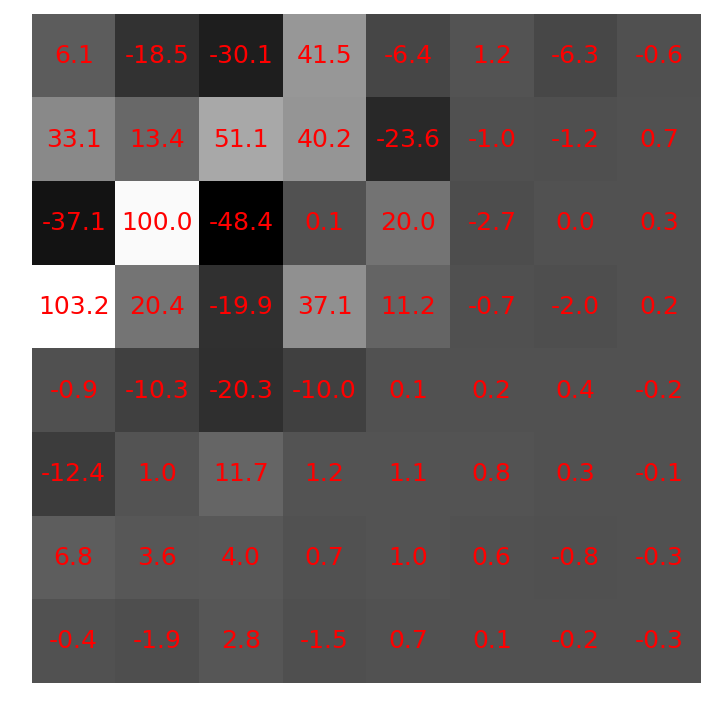
\includegraphics[scale=0.12]{fig/8x8random_dct1.png}
        \hspace{0.5cm}
        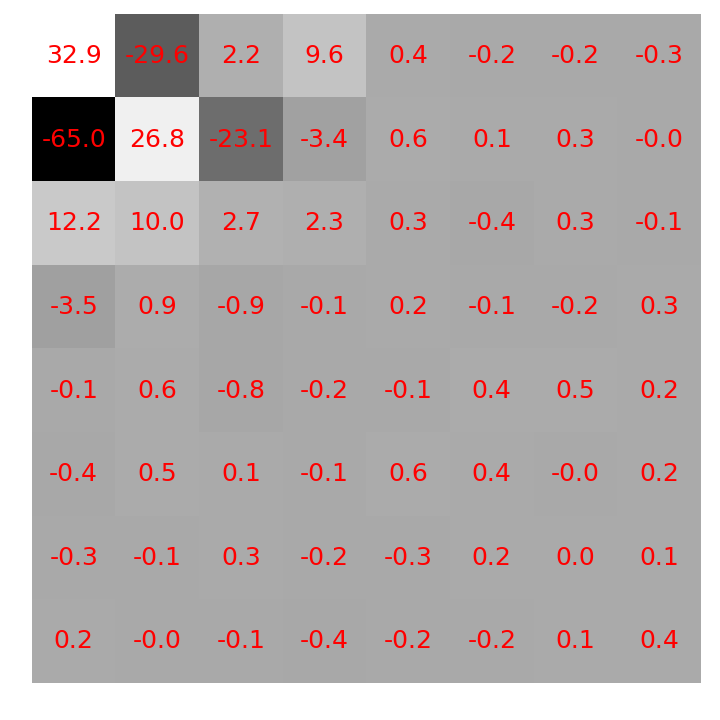
\includegraphics[scale=0.12]{fig/8x8random_dct2.png}
    \end{center}

\end{frame}

\begin{frame}
    % acá vemos cómo se va formando lena a medida que usamos más frecuencias.
    % la imagen 'i' está usando las primeras i frecuencias en ambos sentidos.

    % Vemos como se va formando, y con las primeras 40 frecuencias
    % ya vemos a lena, y son 512 en total. o sea con poquita información
    % guardada podríamos tener una imagen muy aproximada. entonces parecería que
    % aplicar la DCT a la imagen completa funciona! WAIT .... (proxima diapo)
    \begin{columns}
        \column{\dimexpr\paperwidth-10pt}
        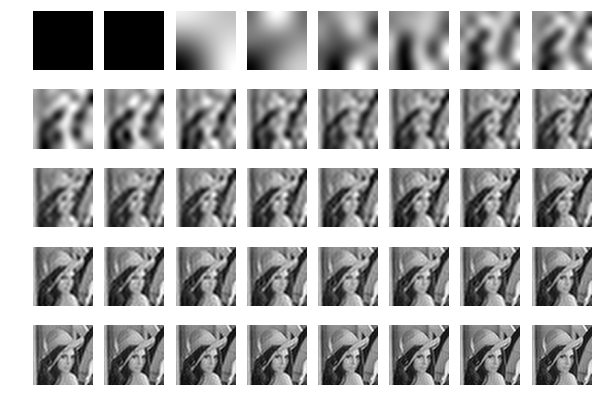
\includegraphics[scale=0.56]{fig/lenas.png}
      \end{columns}

\end{frame}


\begin{frame}
    % acá vemos a lena reconstruina con las priemras 100 frecuencias en ambos
    % sentidos. acá se evidencian los artifacts groseros que produce esto.
    % queda como todo ondulado. esto tiene que ver con el ejemplo de la imagen
    % no homogénea que veiamos: distintas zonas de la imagen tienen distintas
    % frecuencias predominantes, y para obtener dos partes de la imagen distintas
    % bien formadas, necesitamos casi todas las frecuencias
    Reconstrucción de Lena con las 100 frecuencias más bajas en ambos sentidos.
    \begin{center}
        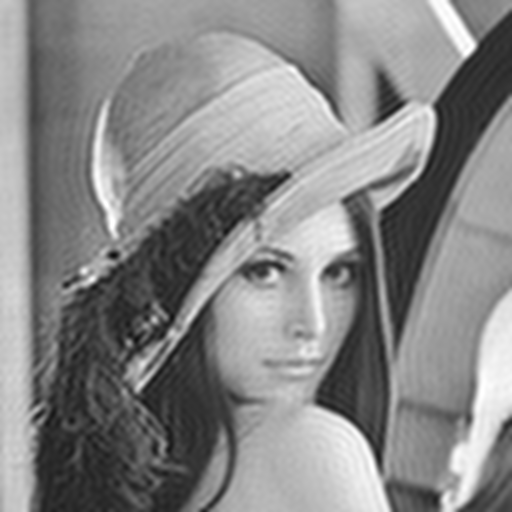
\includegraphics[scale=0.35]{fig/lenas_100frecuencias.png}
    \end{center}
\end{frame}

\subsection{Cuantizar los coeficientes}

\begin{frame}
    \frametitle{3. Cuantizar los coeficientes}
    \begin{itemize}
        \item Dada la matriz de cuantización, reemplazar cada coeficiente de la DCT por
            la división entera entre éste y el de la matriz.
    \end{itemize}

    \vfill

    \begin{minipage}[t]{0.3\linewidth}
        \begin{center}
            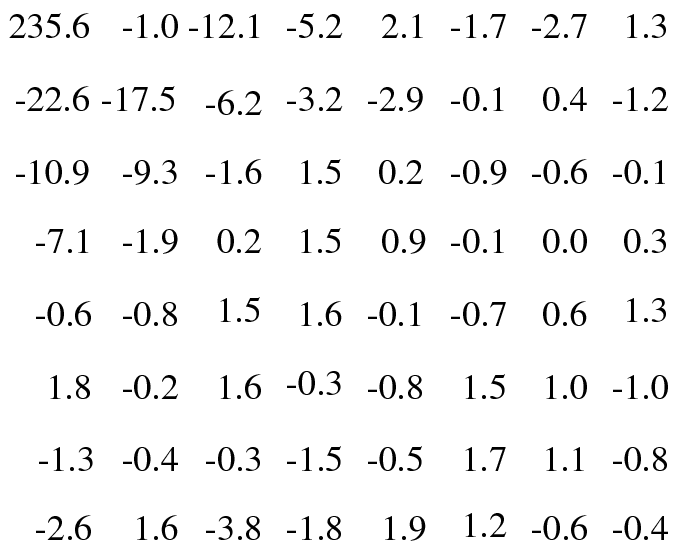
\includegraphics[scale=0.175]{fig/DCT_coefs.png}\\
            \small Coeficientes DCT
        \end{center}
    \end{minipage}
    \hfill
    \begin{minipage}[t]{0.3\linewidth}
        \begin{center}
            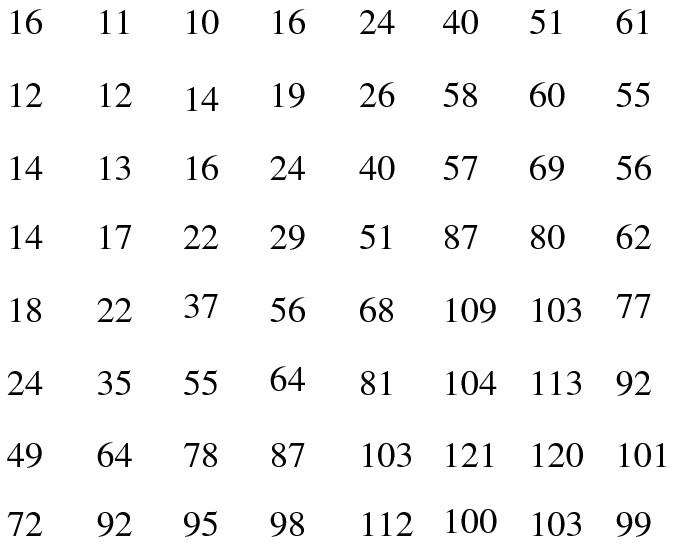
\includegraphics[scale=0.175]{fig/QTable.png}\\
            \small Matriz de cuantización
        \end{center}    \end{minipage}
    \hfill
    \begin{minipage}[t]{0.3\linewidth}
        \begin{center}
            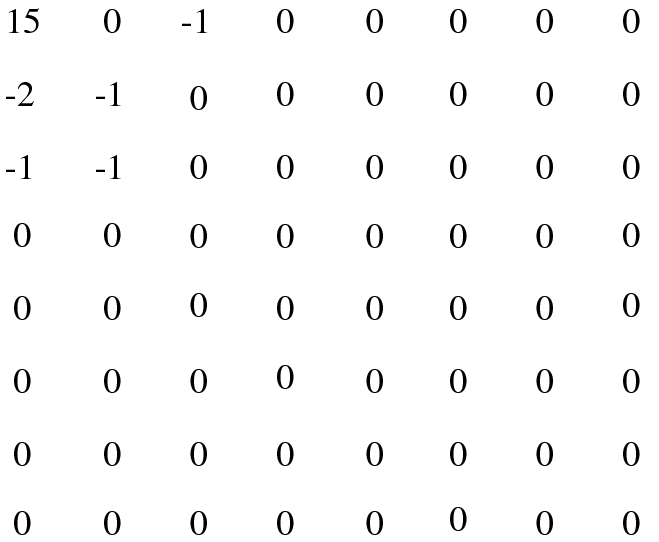
\includegraphics[scale=0.175]{fig/quantized.png}\\
            \small Cociente
        \end{center}    \end{minipage}


\end{frame}


\begin{frame}
    % [TODO] por qué cuantizamos? Para comprimir más y más fácil. bajamos la entropía.
    % Es importante entender que no estamos descartando por frecuencias, sino
    % que estamos estableciendo como un step.
    \textbf{En este paso ocurren dos cosas muy importantes:}
    \begin{enumerate}
        \item La entropía de la información baja drásticamente.
        \item Perdemos información (\textit{lossy compression}).
    \end{enumerate}
\end{frame}

\begin{frame}
    \textbf{Reducción de entropía}

    \begin{minipage}[t]{0.42\linewidth}
        \begin{center}
            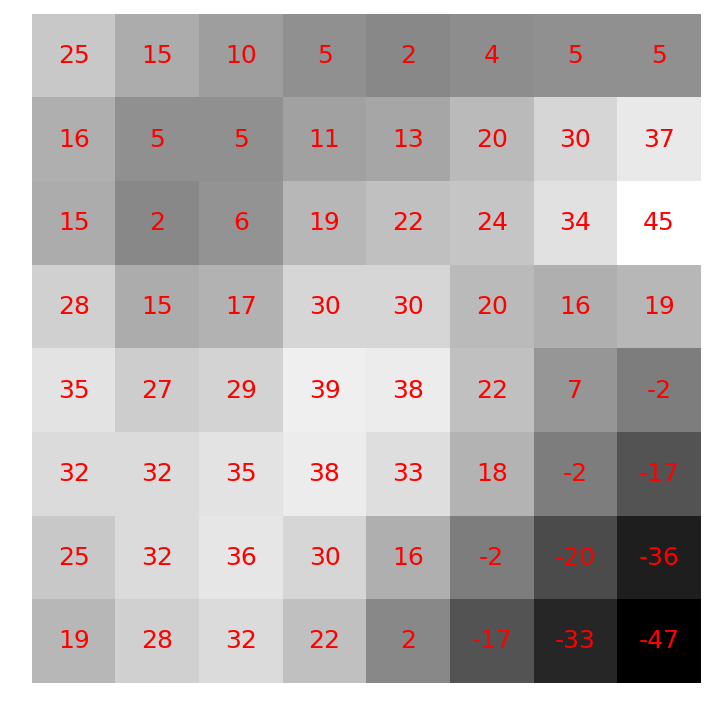
\includegraphics[scale=0.2]{fig/8x8random_entropy.png}\\
            4,935
        \end{center}
    \end{minipage}
    \hfill
    \begin{minipage}[t]{0.42\linewidth}
        \begin{center}
            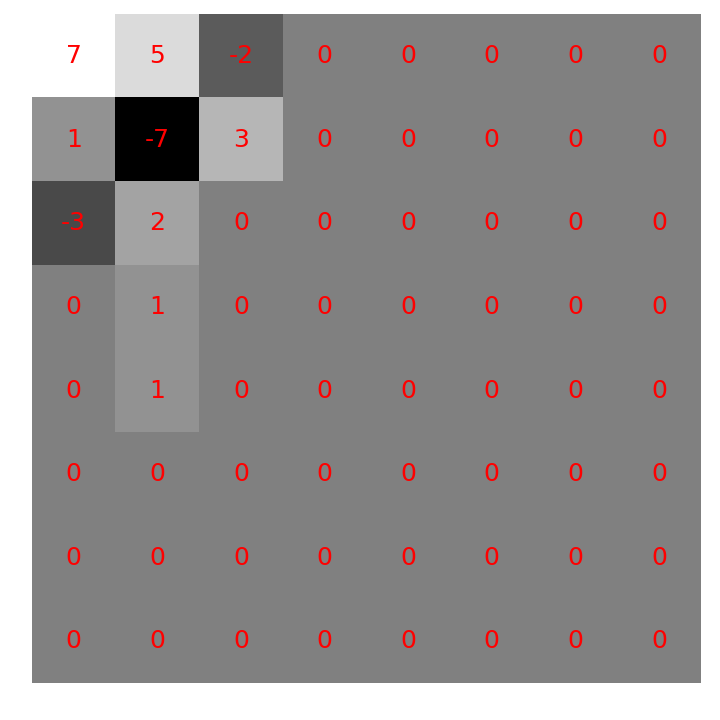
\includegraphics[scale=0.2]{fig/8x8random_dct_entropy.png}\\
            1,07
        \end{center}
    \end{minipage}
\end{frame}

\begin{frame}
    \textbf{Reducción de entropía}
    
    \begin{minipage}[t]{0.42\linewidth}
        \begin{center}
            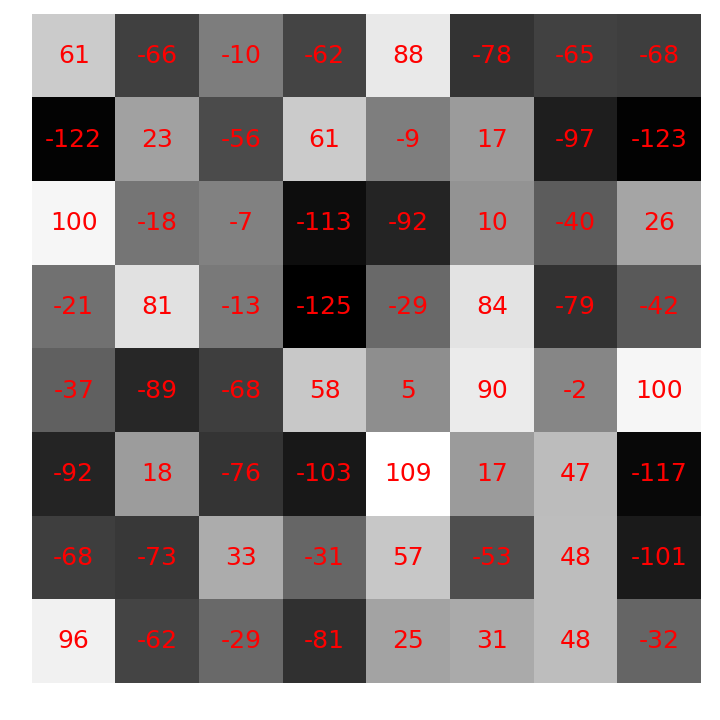
\includegraphics[scale=0.2]{fig/8x8random_entropy2.png}\\
            5,707
        \end{center}
    \end{minipage}
    \hfill
    \begin{minipage}[t]{0.42\linewidth}
        \begin{center}
            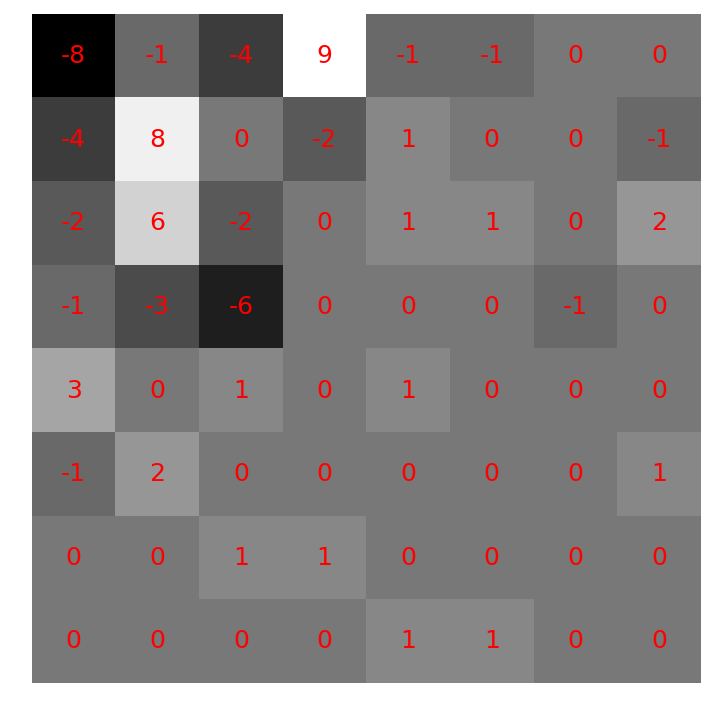
\includegraphics[scale=0.2]{fig/8x8random_dct_entropy2.png}\\
            2,436
        \end{center}
    \end{minipage}
\end{frame}

\begin{frame}
    \frametitle{Artifacts}
    % el artifact más común se da en los bordes, por la eliminación de frecuencias
    % bajas
    \begin{minipage}[t]{0.4\linewidth}
        \begin{center}
            
\includegraphics[width=4cm, height=4cm]{fig/borde.png}\\
            Imagen original
        \end{center}
    \end{minipage}
    \hfill
    \begin{minipage}[t]{0.4\linewidth}
        \begin{center}
        
\includegraphics[width=4cm, height=4cm]{fig/borde_jpeg.png}\\
        Imagen comprimida con JPEG
        \end{center}
    \end{minipage}
\end{frame}

\begin{frame}
    %\centering Artifacts en imágenes texto
    \begin{minipage}[t]{0.4\linewidth}
        \begin{center}
            {
                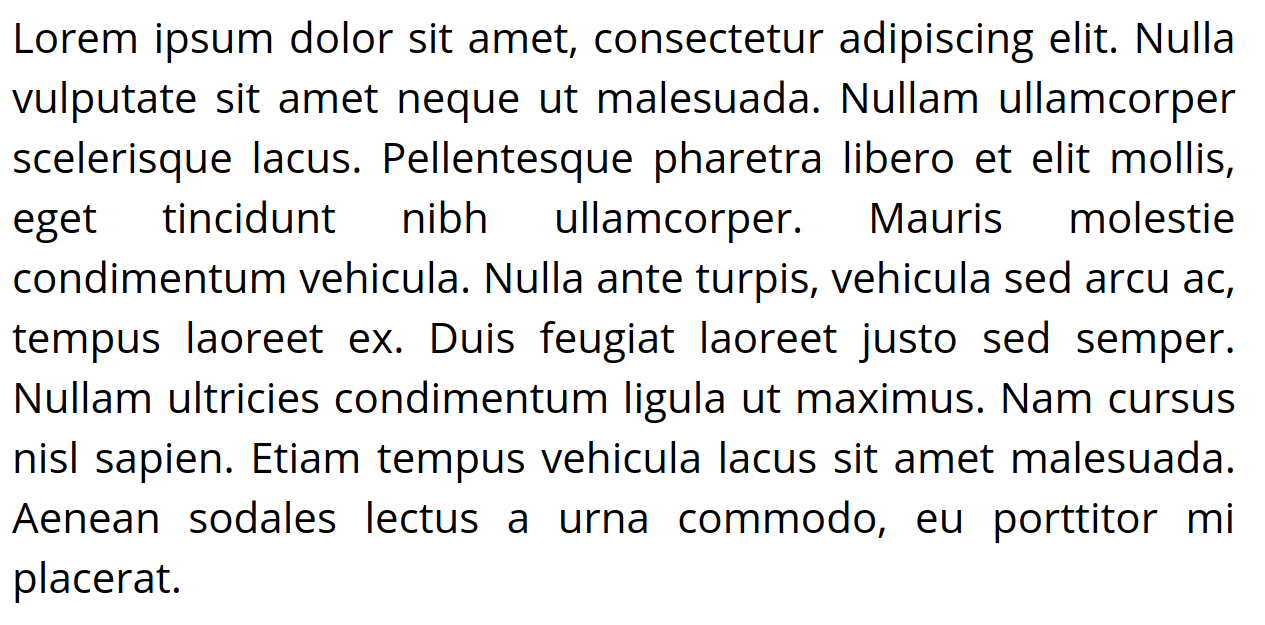
\includegraphics[width=5cm]{fig/text.png}\\
                Imagen original
            }
        \end{center}
    \end{minipage}
    \hfill
    \begin{minipage}[t]{0.4\linewidth}
        % NOTE: con calidad Q=100
        % NOTE2: no pude centrarlo, paja
        \begin{center}
            {
                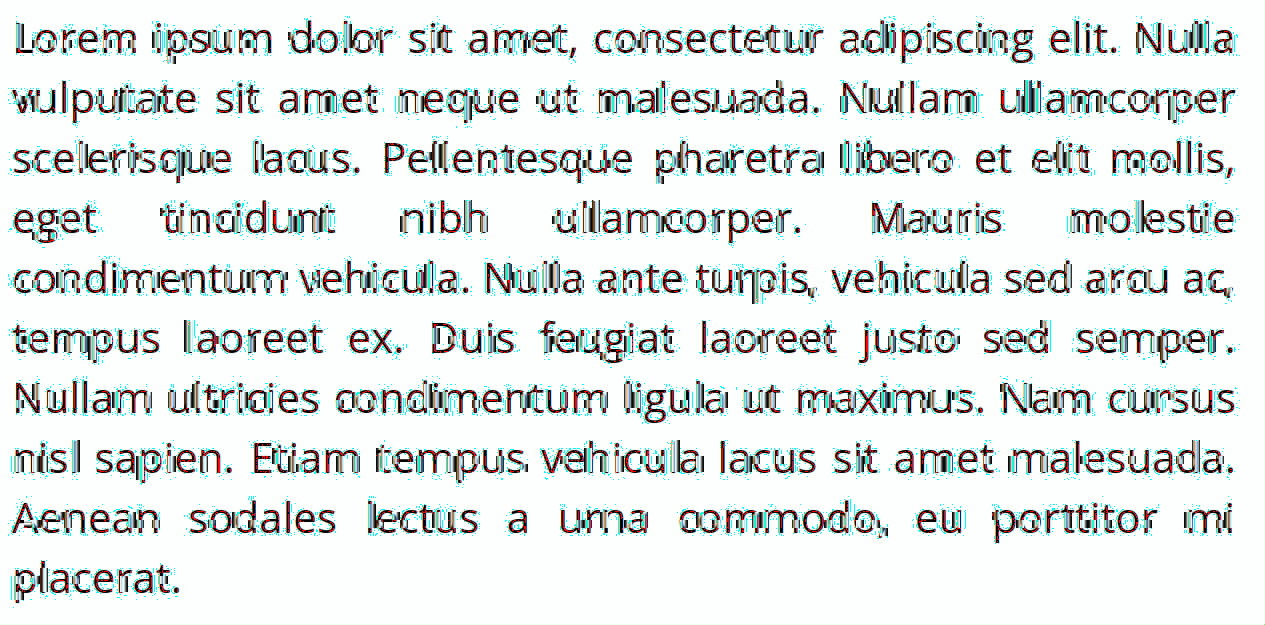
\includegraphics[width=5cm]{fig/text_artifacts.png}\\
                Imagen comprimida con JPEG
            }
        \end{center}
    \end{minipage}
\end{frame}

\subsection{Compresión entrópica}
\begin{frame}
    % ahora que bajamos mucho la entropía podemos comprimir mucho más.
    % aca presentamos una versión un poco simplificada. la estándar es muy
    % parecida, pero difiere en la parte de tuplas/huffman. no corre huffman
    % cada vez sino que tiene un diccionario guardado, y lo usa sobre otras tuplas
    % La codificación entrópica típica de JPEG se puede dividir en 4 pasos:
    \frametitle{4. Comprimir el conjunto de coeficientes finales}
    \begin{enumerate}
        \item Codificar los coeficientes DC
        \item Desarmar en $zig-zag$ cada cuadrado
        \item Comprimir cada cuadrado como tuplas $(\# ceros \, antes, \, valor)$
        \item Codificar las tuplas con Huffman
    \end{enumerate}
\end{frame}

\begin{frame}
    \begin{enumerate}
        \item Codificar los coeficientes DC: el coeficiente DC de cada bloque se guarda como su diferencia con el del bloque anterior.
        \item Desarmar en $zig-zag$ cada cuadrado: se arma una secuencia por bloque recorriéndolo en $zig-zag$.
    \end{enumerate}
    \vfill
    \begin{minipage}[t]{0.3\linewidth}
        \begin{center}
        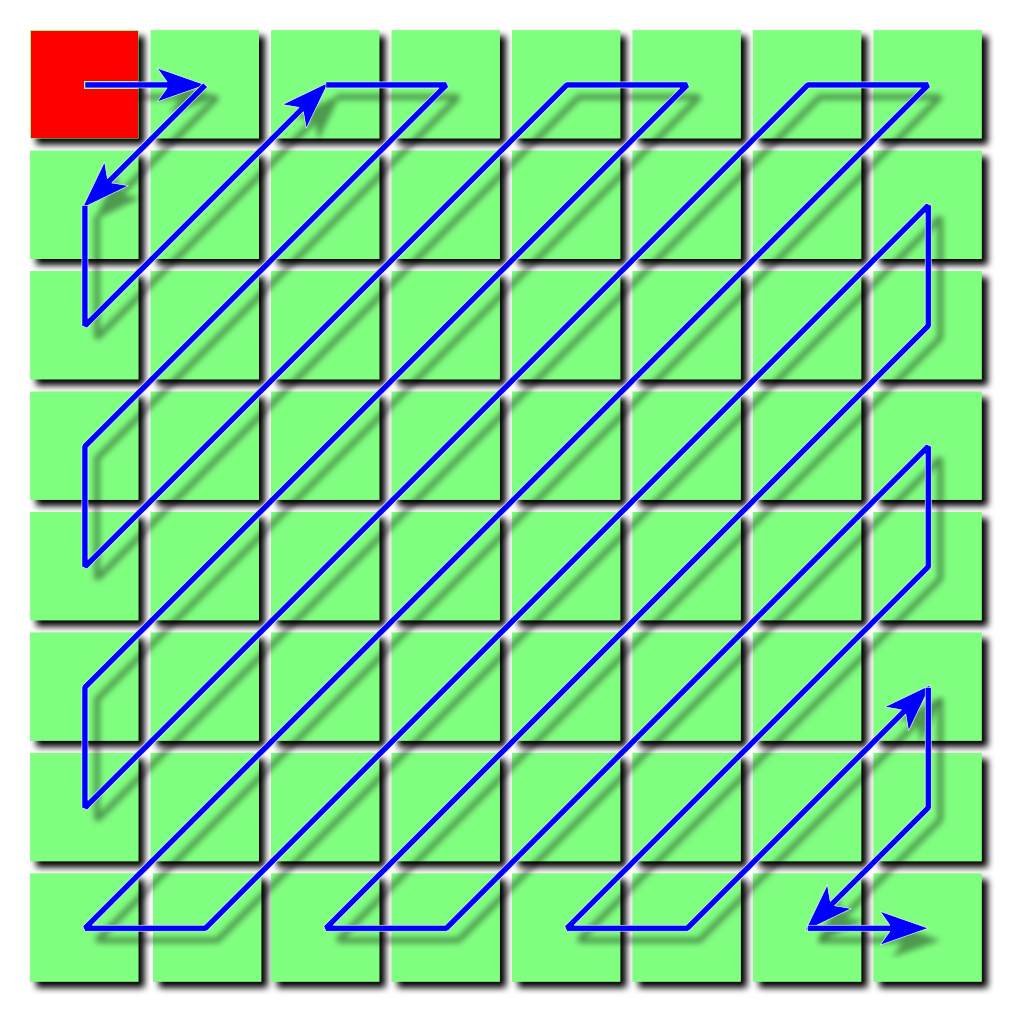
\includegraphics[scale=0.10]{fig/zigzag_dc.png}\\
        \small Bloque 0
        \end{center}
    \end{minipage}
    \hfill
    \begin{minipage}[t]{0.3\linewidth}
        \begin{center}
        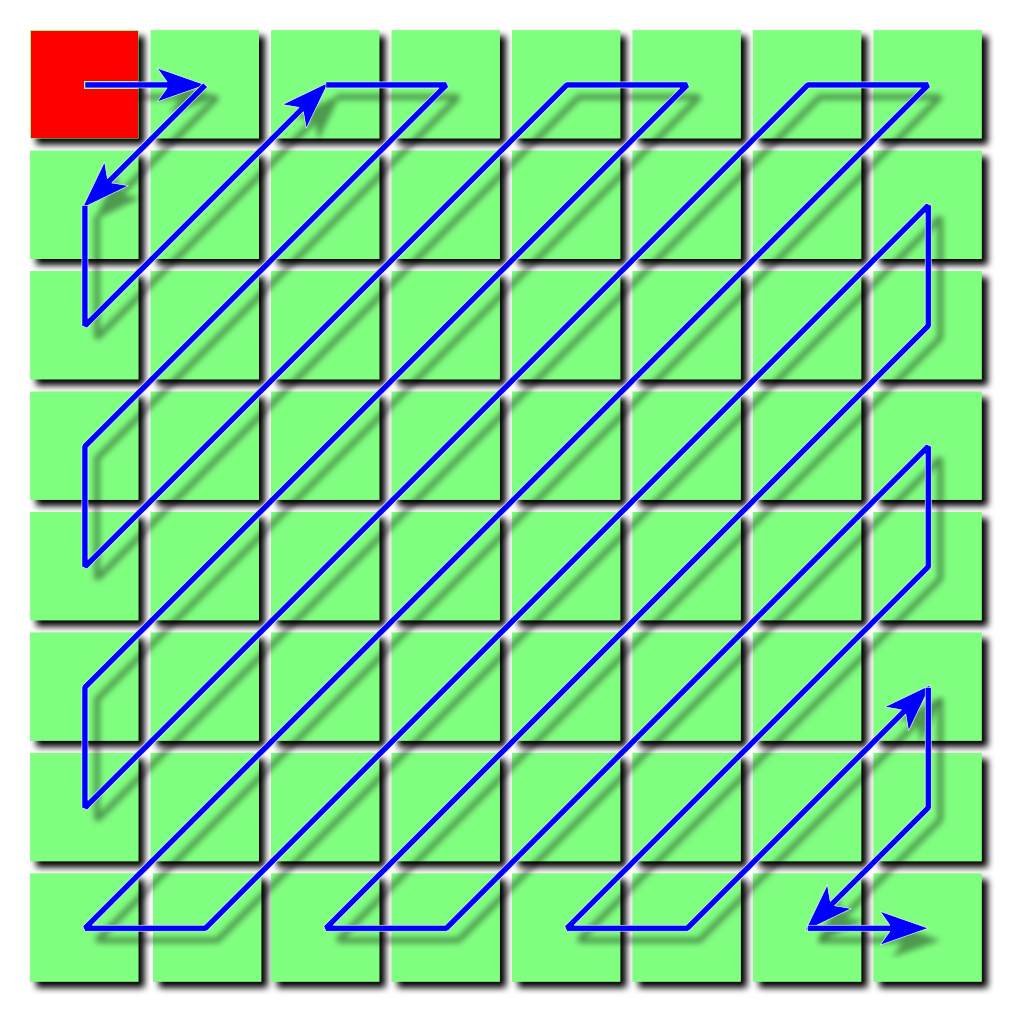
\includegraphics[scale=0.10]{fig/zigzag_dc.png}\\
        \small Bloque 1
        \end{center}
    \end{minipage}
    \hfill
    \begin{minipage}[t]{0.3\linewidth}
        \begin{center}
        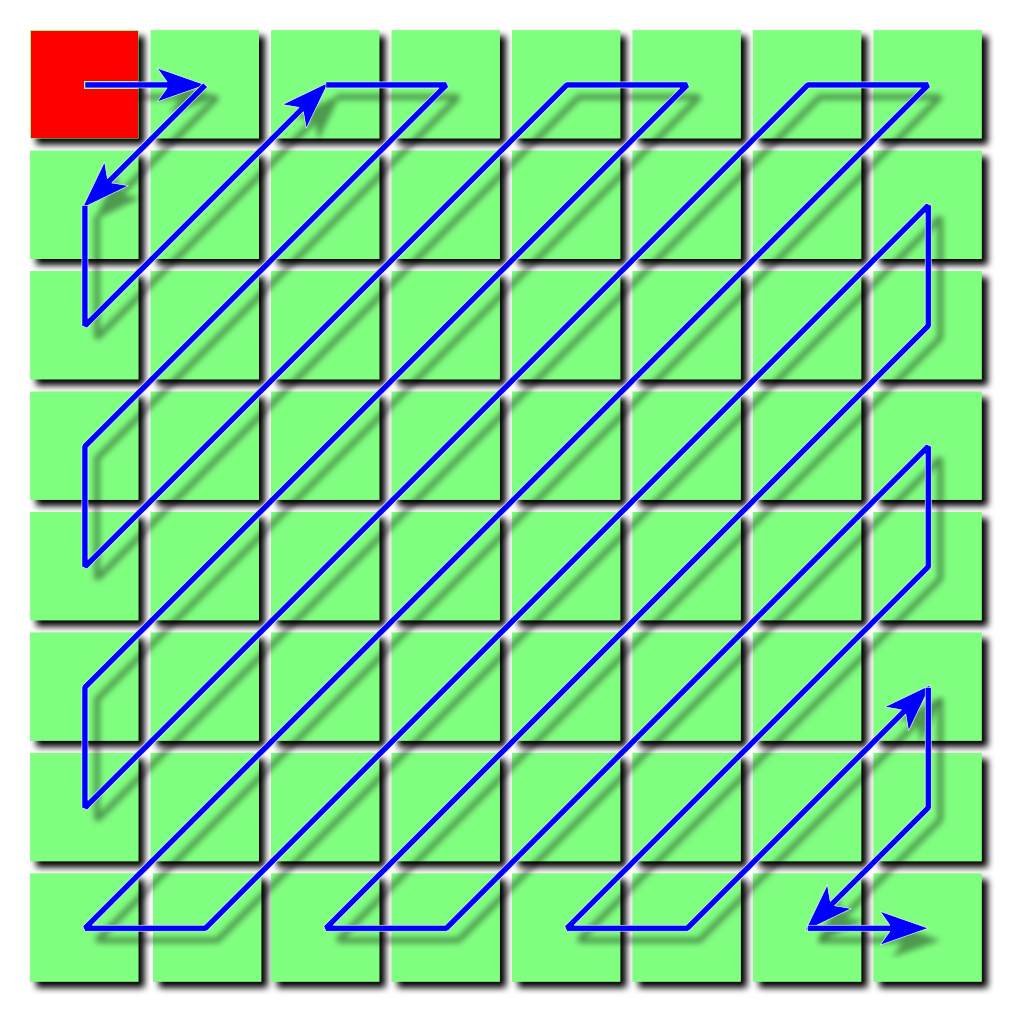
\includegraphics[scale=0.10]{fig/zigzag_dc.png}\\
        \small Bloque 2
        \end{center}
    \end{minipage}
\end{frame}


\begin{frame}
    \begin{enumerate}\addtocounter{enumi}{2}
        \item Comprimir cada cuadrado como tuplas $(\# ceros \, antes, \, valor)$: cada secuencia del paso anterior de codifica con tuplas que comprimen ceros consecutivos.

        \item Codificar las tuplas con Huffman.
    \end{enumerate}

    \vfill
    \begin{center}
        \textbf{15}, {\color{red} 0}, $-2$, 7, $-1$, $-1$, {\color{red} 0}, {\color{red} 0}, $-1$, {\color{red} 0}, {\color{red} 0}, {\color{red} 0}, {\color{red} 0}, {\color{red} 0}, {\color{red} 0}, {\color{red} 0}, 5, {\color{red} 0}, {\color{red} 0}, ... , {\color{red} 0}

        \vfill
        $\downarrow$

        {\tiny compresión a tuplas}
        \vfill

        (\textbf{15}) ({\color{red}1},$-2$) ({\color{red}0},7) ({\color{red}0},$-1$) ({\color{red}0},$-1$) ({\color{red}2},$-1$) ({\color{red}7},5) {\color{red}(0,0)}

        \vfill
        $\downarrow$

        {\tiny codificación con Huffman}
        \vfill

        1000111010000111010110 (22 bits)
    \end{center}
\end{frame}

\begin{frame}
    \begin{center}
        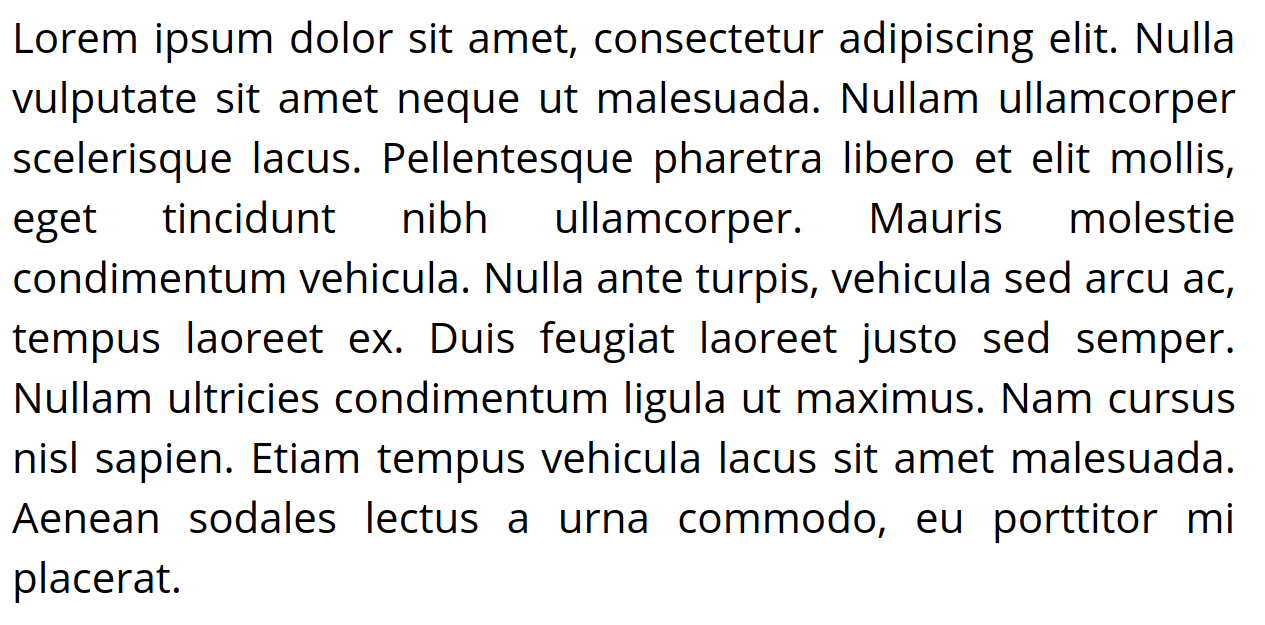
\includegraphics[scale=0.15]{fig/text.png}

        \vfill

        \hfill
        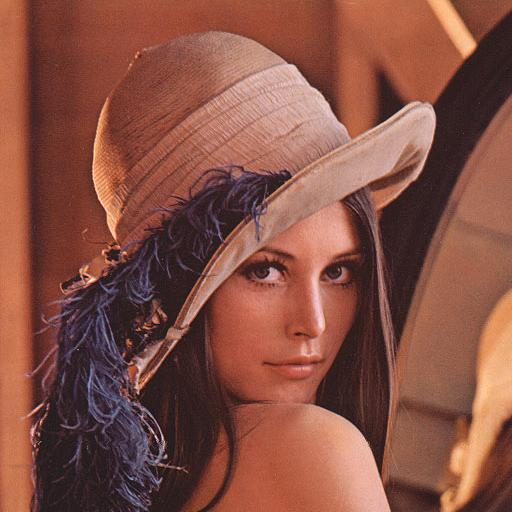
\includegraphics[scale=0.25]{fig/lena.jpg}
        \hfill
        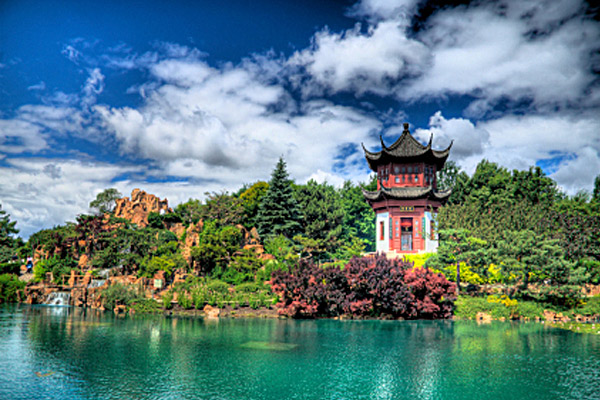
\includegraphics[scale=0.25]{fig/landscape.jpg}
        \hfill
    \end{center}
\end{frame}

\begin{frame}
    \begin{center}
        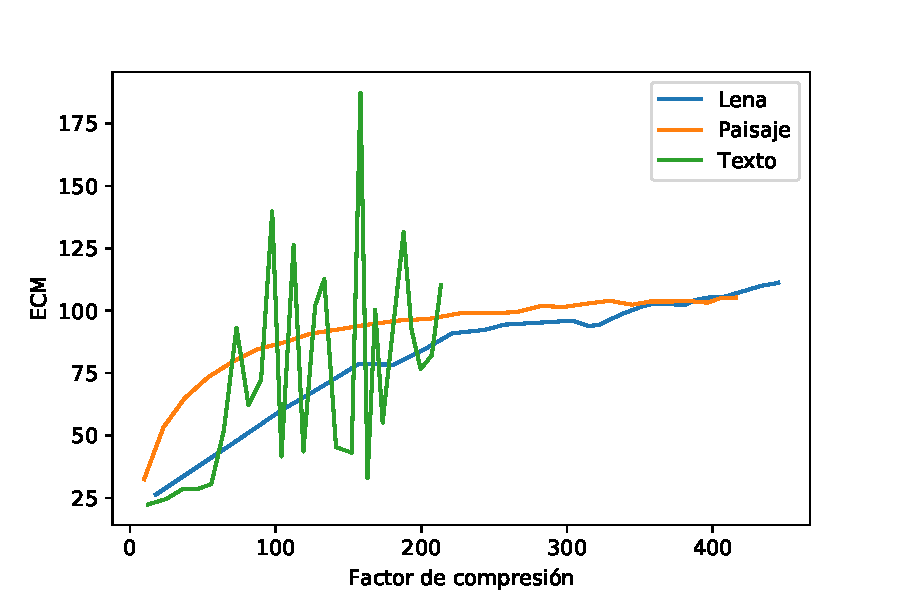
\includegraphics[scale=0.7]{fig/FCvsECM.pdf}
    \end{center}
\end{frame}

\begin{frame}
    \begin{center}

        \hfill
        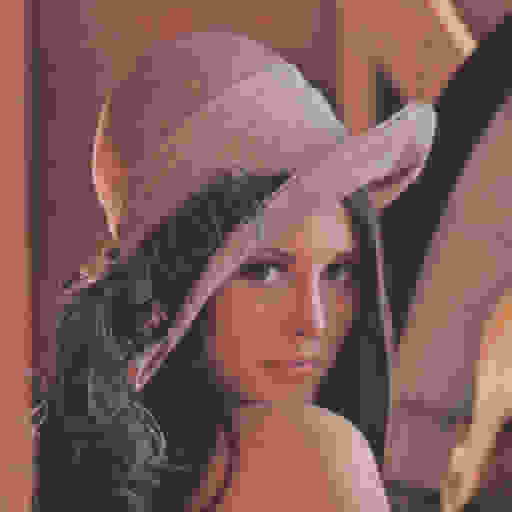
\includegraphics[scale=0.2]{fig/lena_80.png}
        \hfill
        %         94.4124298096
        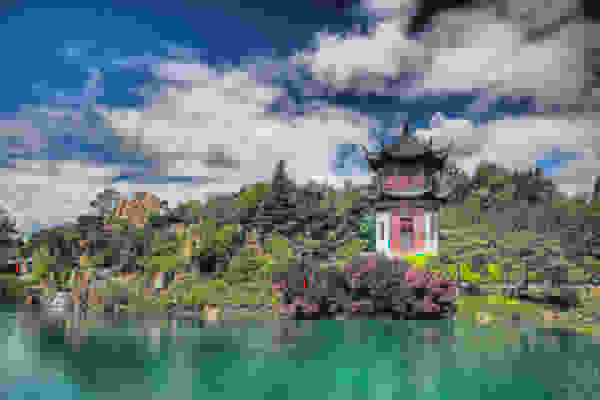
\includegraphics[scale=0.2]{fig/paisaje_80.png}
        % 96.0637166667
        \hfill

        \vfill
        {\small ECM $\sim 100$}

    \end{center}
\end{frame}


\begin{frame}
    \begin{center}
        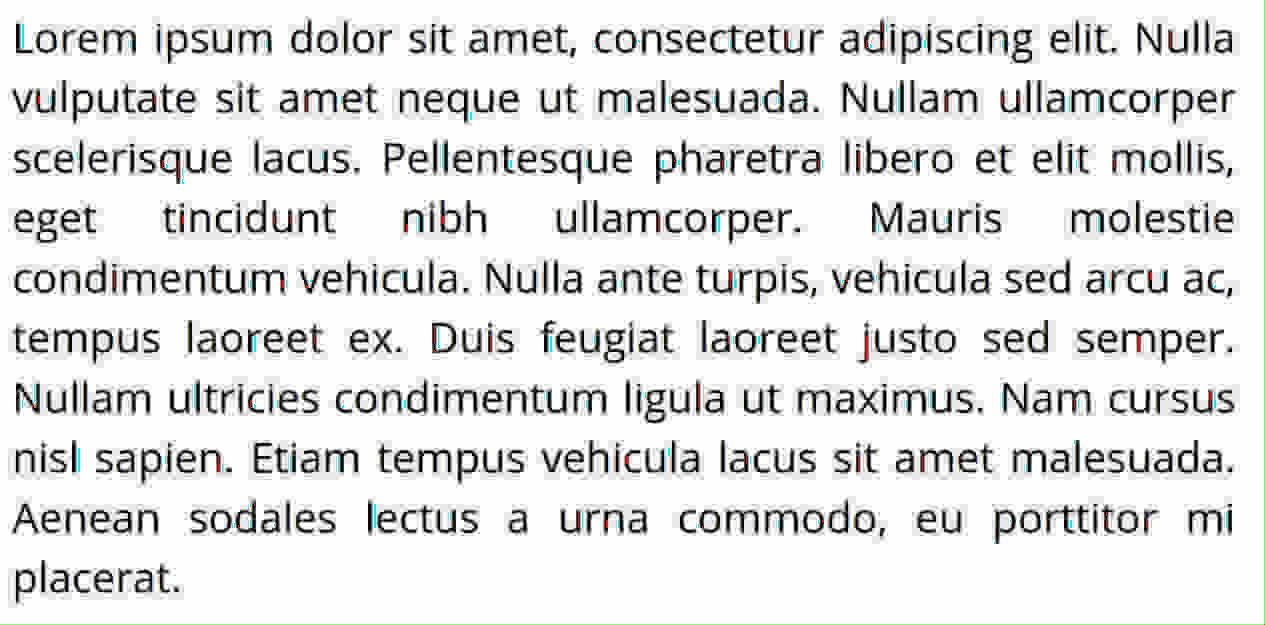
\includegraphics[scale=0.2]{fig/txt_80.png}


        \vfill
        {\small ECM $\sim 40$}

    \end{center}

\end{frame}


\section{Resumen}
\begin{frame}
    \frametitle{Resumiendo}
    \begin{center}
        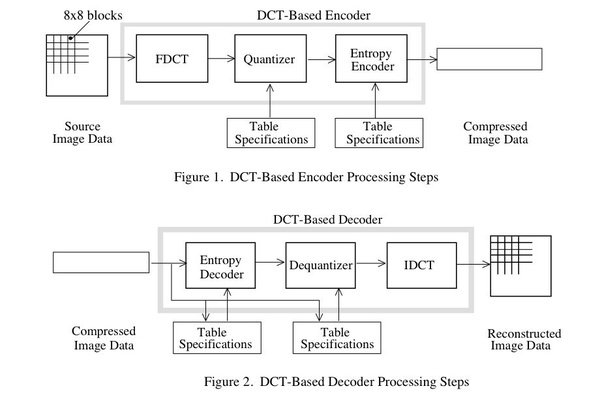
\includegraphics[scale=0.45]{fig/steps.jpeg}
    \end{center}
\end{frame}

\begin{frame}
    \begin{center}
        \textit{this$\rightarrow$context\_switch('ruido')}
    \end{center}
\end{frame}

\section{Ruido}    
\begin{frame}
    \frametitle{¿Cómo cambia la compresión de una imagen con ruido?}
    \vspace{0mm}
    \pause

    \noindent\makebox[\linewidth][c]{%
    \begin{minipage}[t]{0.42\linewidth}
        \begin{center}
            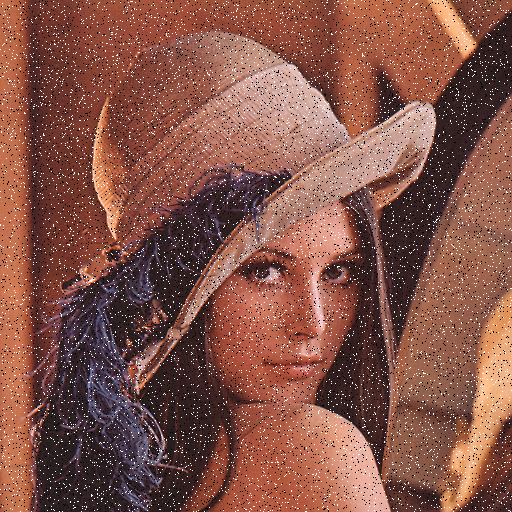
\includegraphics[scale=0.3]{fig/lena_contaminada.png}\\
        \end{center}
    \end{minipage}
    \hfill
    \begin{minipage}[t]{0.42\linewidth}
        \begin{itemize}
            \item Ruido $\rightarrow$ frecuencias altas
            \pause
            \item Mayor coeficiente en frecuencias altas $\Rightarrow$ menor compresibilidad
            \pause
            \item Si fuera puntual, afectaría a un solo bloque. Al estar disperso, la totalidad de
                la imagen se ve afectada
        \end{itemize}
    \end{minipage}
    }

\end{frame}


% TODO: Agregar 'conclusiones' de esto del ruido
\begin{frame}
    \framesubtitle{¿Qué medimos?}
    $FC_{\text{imagen contaminada}} - FC_{\text{imagen original}}$\\
    \vspace{3mm}
    para distintos factores de calidad\\
    \vspace{3mm}
    para distintas distribuciones del ruido
\end{frame}

\begin{frame}
    \begin{center}
        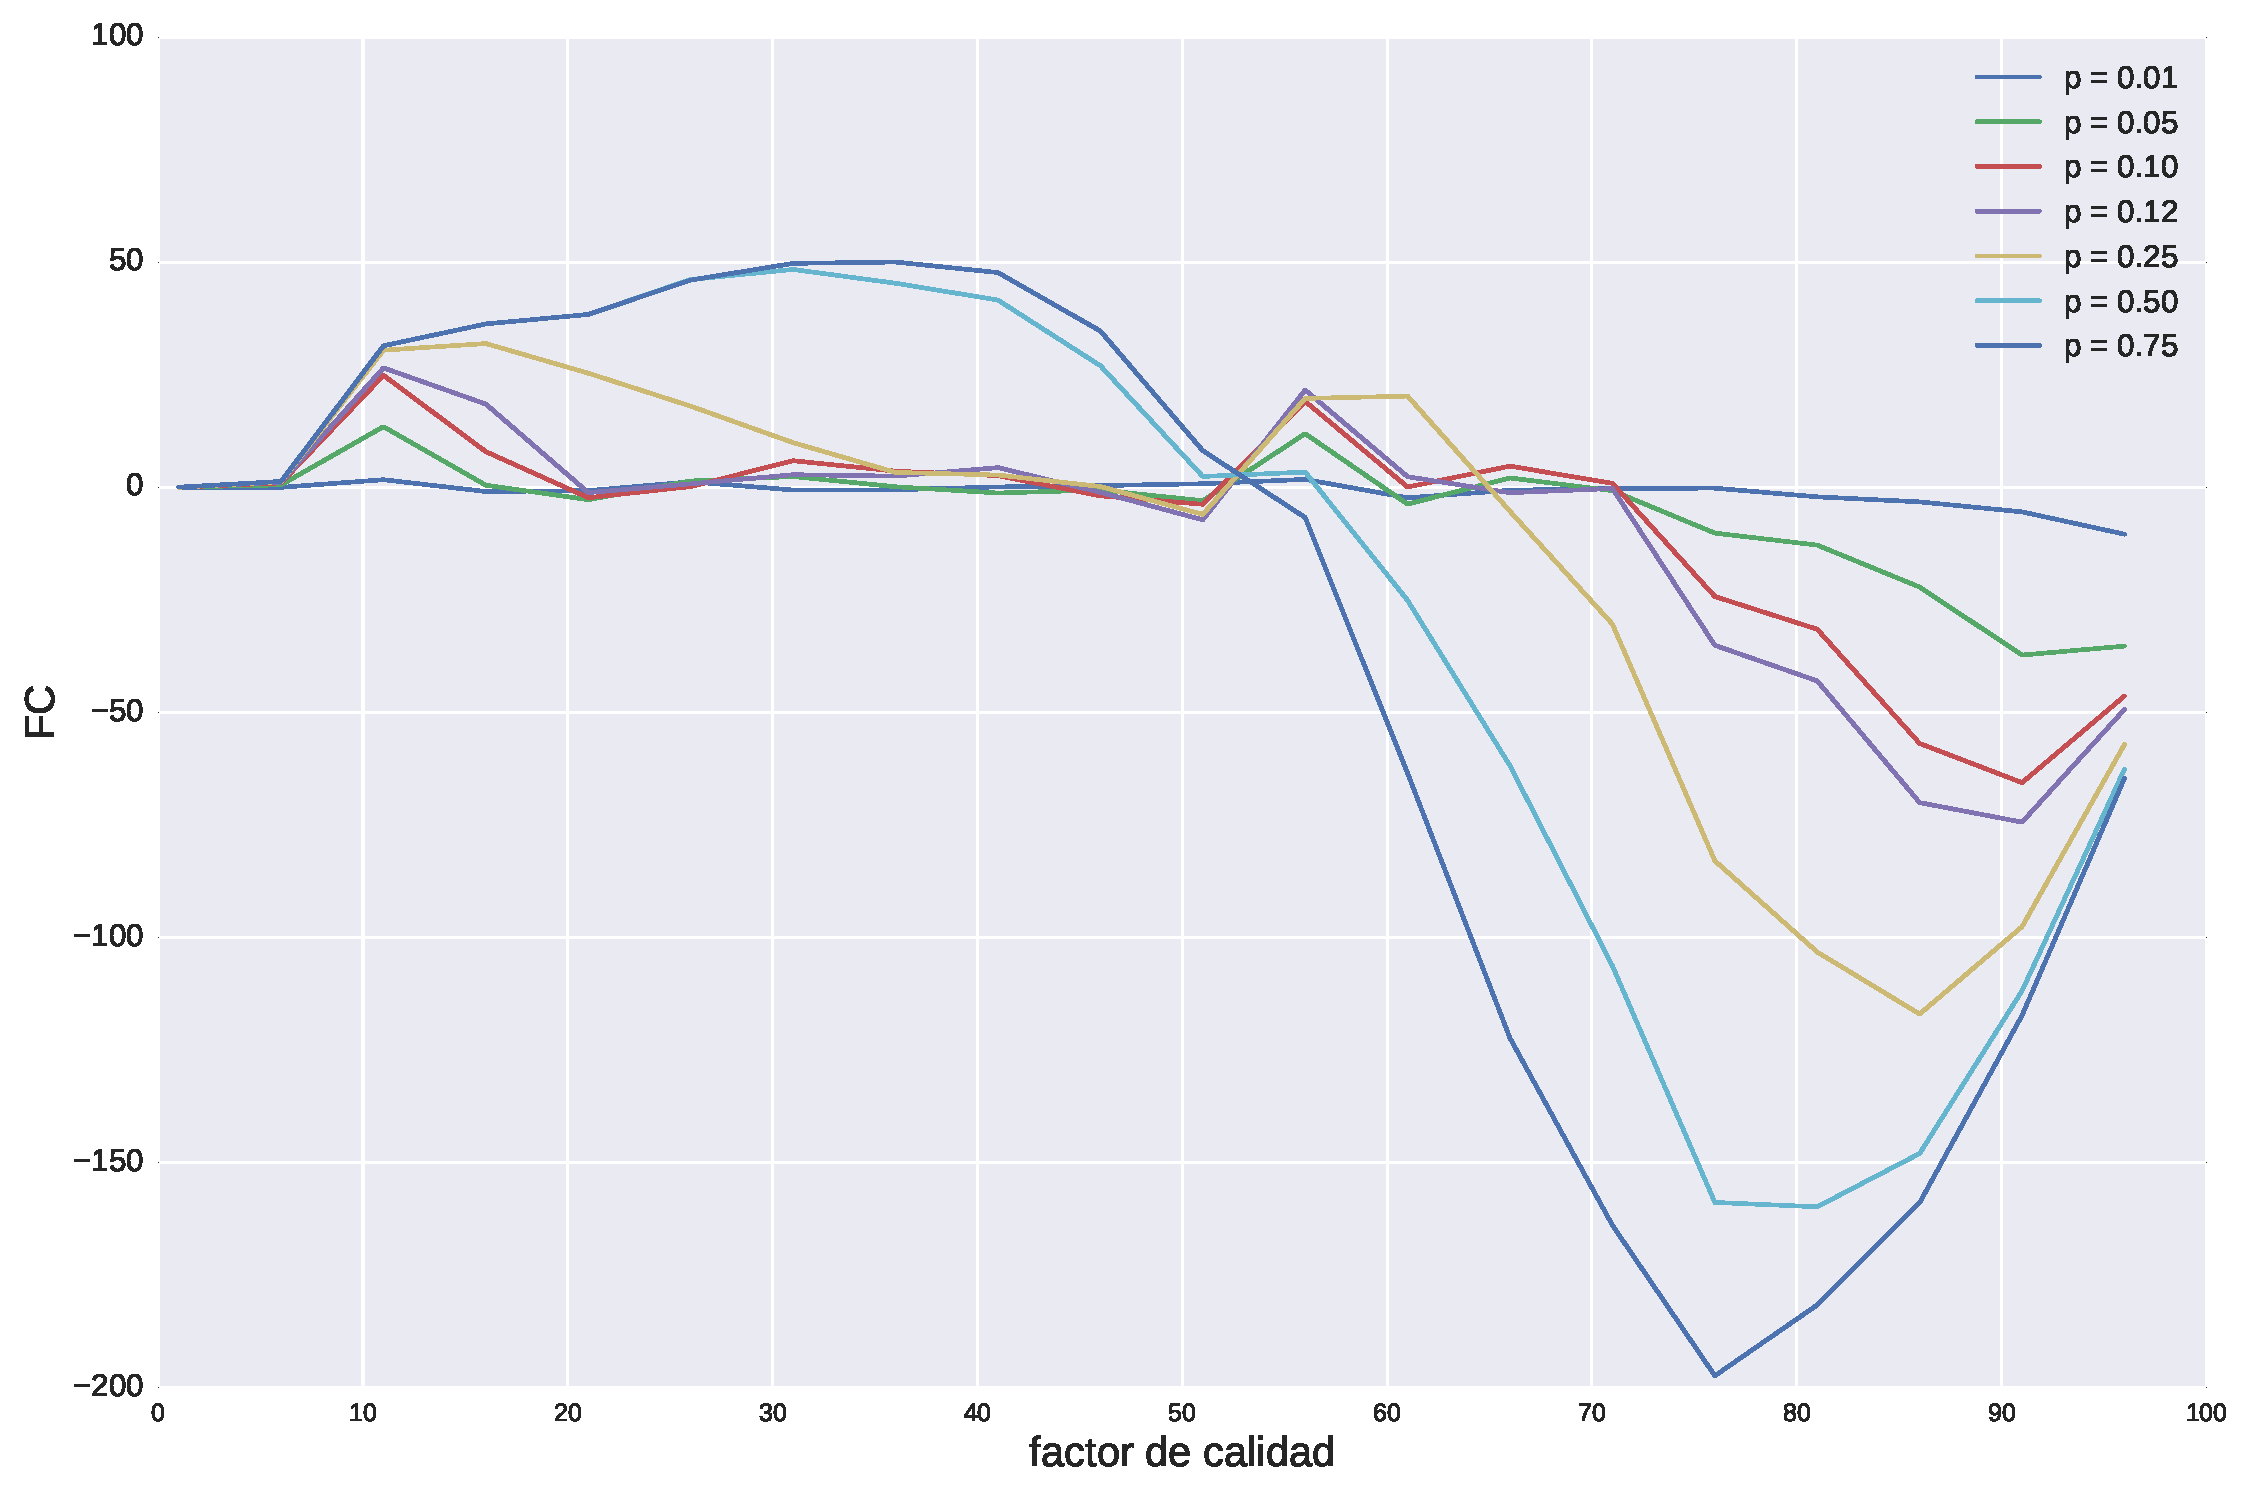
\includegraphics[scale=0.2]{fig/lena_SP_plot.pdf} \\
        \vspace{3mm}
        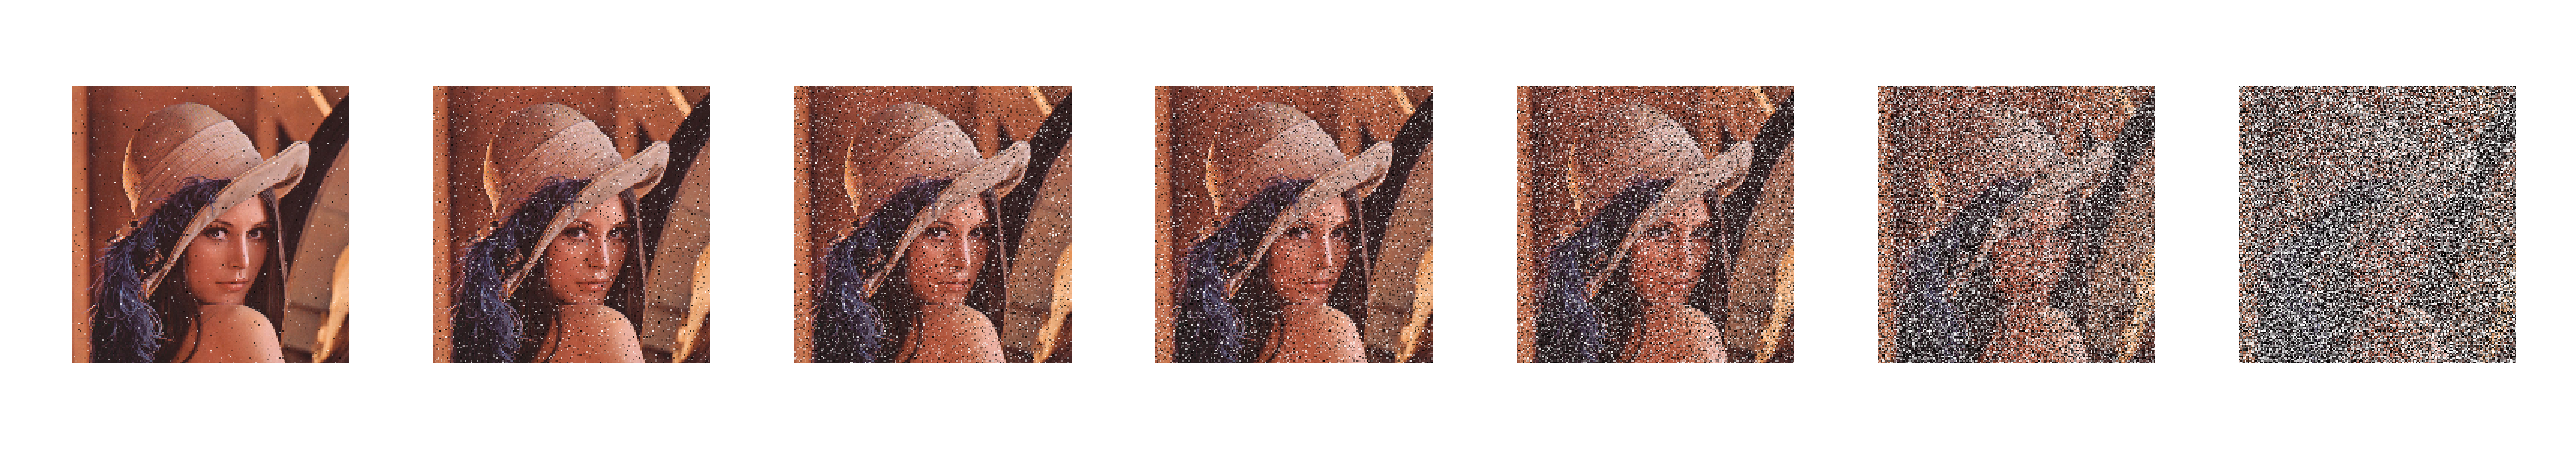
\includegraphics[scale=0.2]{fig/lenas_SP_images.pdf}
    \end{center}
\end{frame}

\begin{frame}
    \begin{center}
        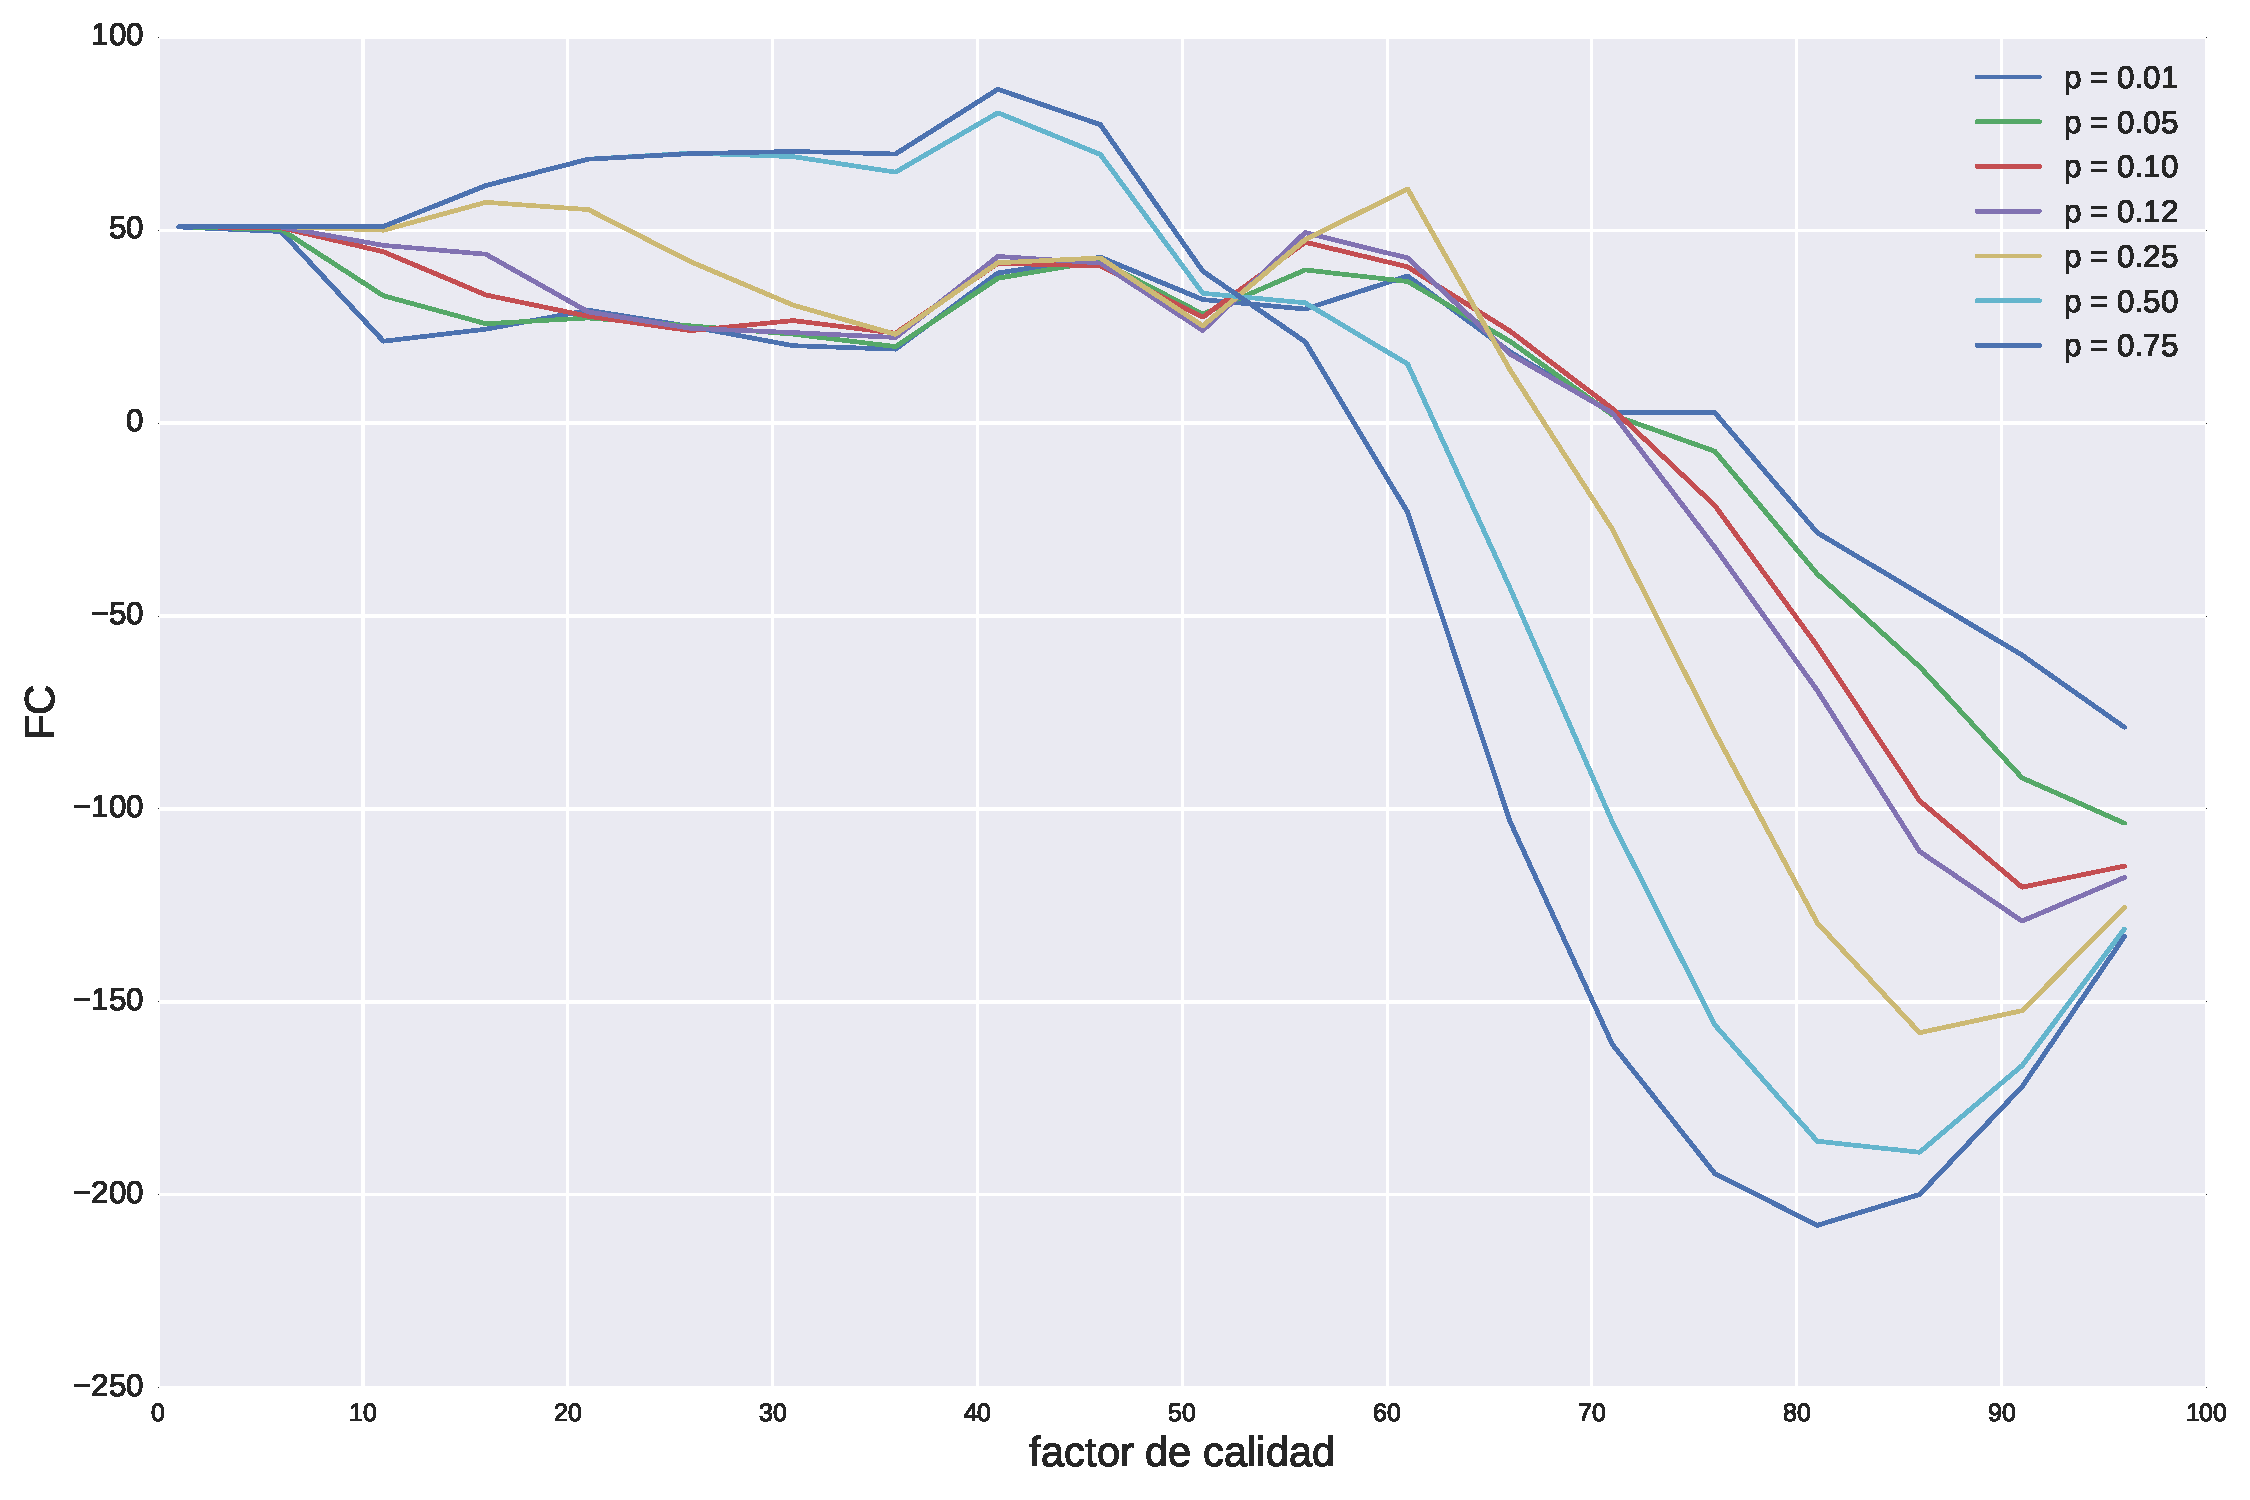
\includegraphics[scale=0.2]{fig/formas_SP_plot.pdf} \\
        \vspace{3mm}
        
\includegraphics[scale=0.2]{fig/formas_SP_images.pdf}
    \end{center}
\end{frame}

\begin{frame}
    % TODO: Agregar 'conclusiones' de esto del ruido
\end{frame}

\begin{frame}
    \begin{center}
        \LARGE\textbf{¿Preguntas?} \\
        \vspace{3mm}
        
\includegraphics[scale=0.2]{fig/preguntas.jpg}
    \end{center}
\end{frame}

\begin{frame}
    \begin{center}
        \huge\textbf{¡Gracias!}
    \end{center}
\end{frame}

\end{document}
